\documentclass[16pt]{beamer}

\usepackage[utf8]{inputenc}
\usepackage[main=russian, english]{babel}
\usepackage{amssymb}
\usepackage{graphicx}

\usetheme{Warsaw}

\title[Конференция <<Ломоносовские чтения 2023>>]
        {Математическое моделирование движения руки и поведенческих движений}
\author[К. Ю. Егоров]
        {студент 2 курса магистратуры К. Ю. Егоров\\
        научный руководитель --- к.ф-м.н., доцент И. В. Востриков}
\institute{Кафедра системного анализа\\ ВМК МГУ}
\date{5 апреля 2023}

% Добавляем в панель навигации номер страницы
\setbeamertemplate{navigation symbols}{
        \insertslidenavigationsymbol
        \insertframenavigationsymbol
        \insertsubsectionnavigationsymbol
        \insertsectionnavigationsymbol
        \insertdocnavigationsymbol
        \insertbackfindforwardnavigationsymbol
        \hspace{1em}
        \usebeamerfont{footline}
        \insertframenumber /\inserttotalframenumber
        %
}

\begin{document}
    \begin{frame}
        \titlepage
    \end{frame}

    \begin{frame}{Введение}
        В работе приведен анализ движения руки человека:
        \begin{itemize}
            \item Построена математическая модель
            \item Поставлена задача оптимального управления для достижения целевого положения руки
            \item Предложен итеративный алгоритм синтеза управления
        \end{itemize}
        \vfill
        \begin{block}{Возможные применения}
            \begin{itemize}
                \item Разработка \textit{умных} протезов
                \item Разработка устройств для управления, корректирования движений людей с болезнями нервной системы
            \end{itemize}
            
        \end{block}
    \end{frame}

    \begin{frame}{Математическое моделирование}
        \centering{
            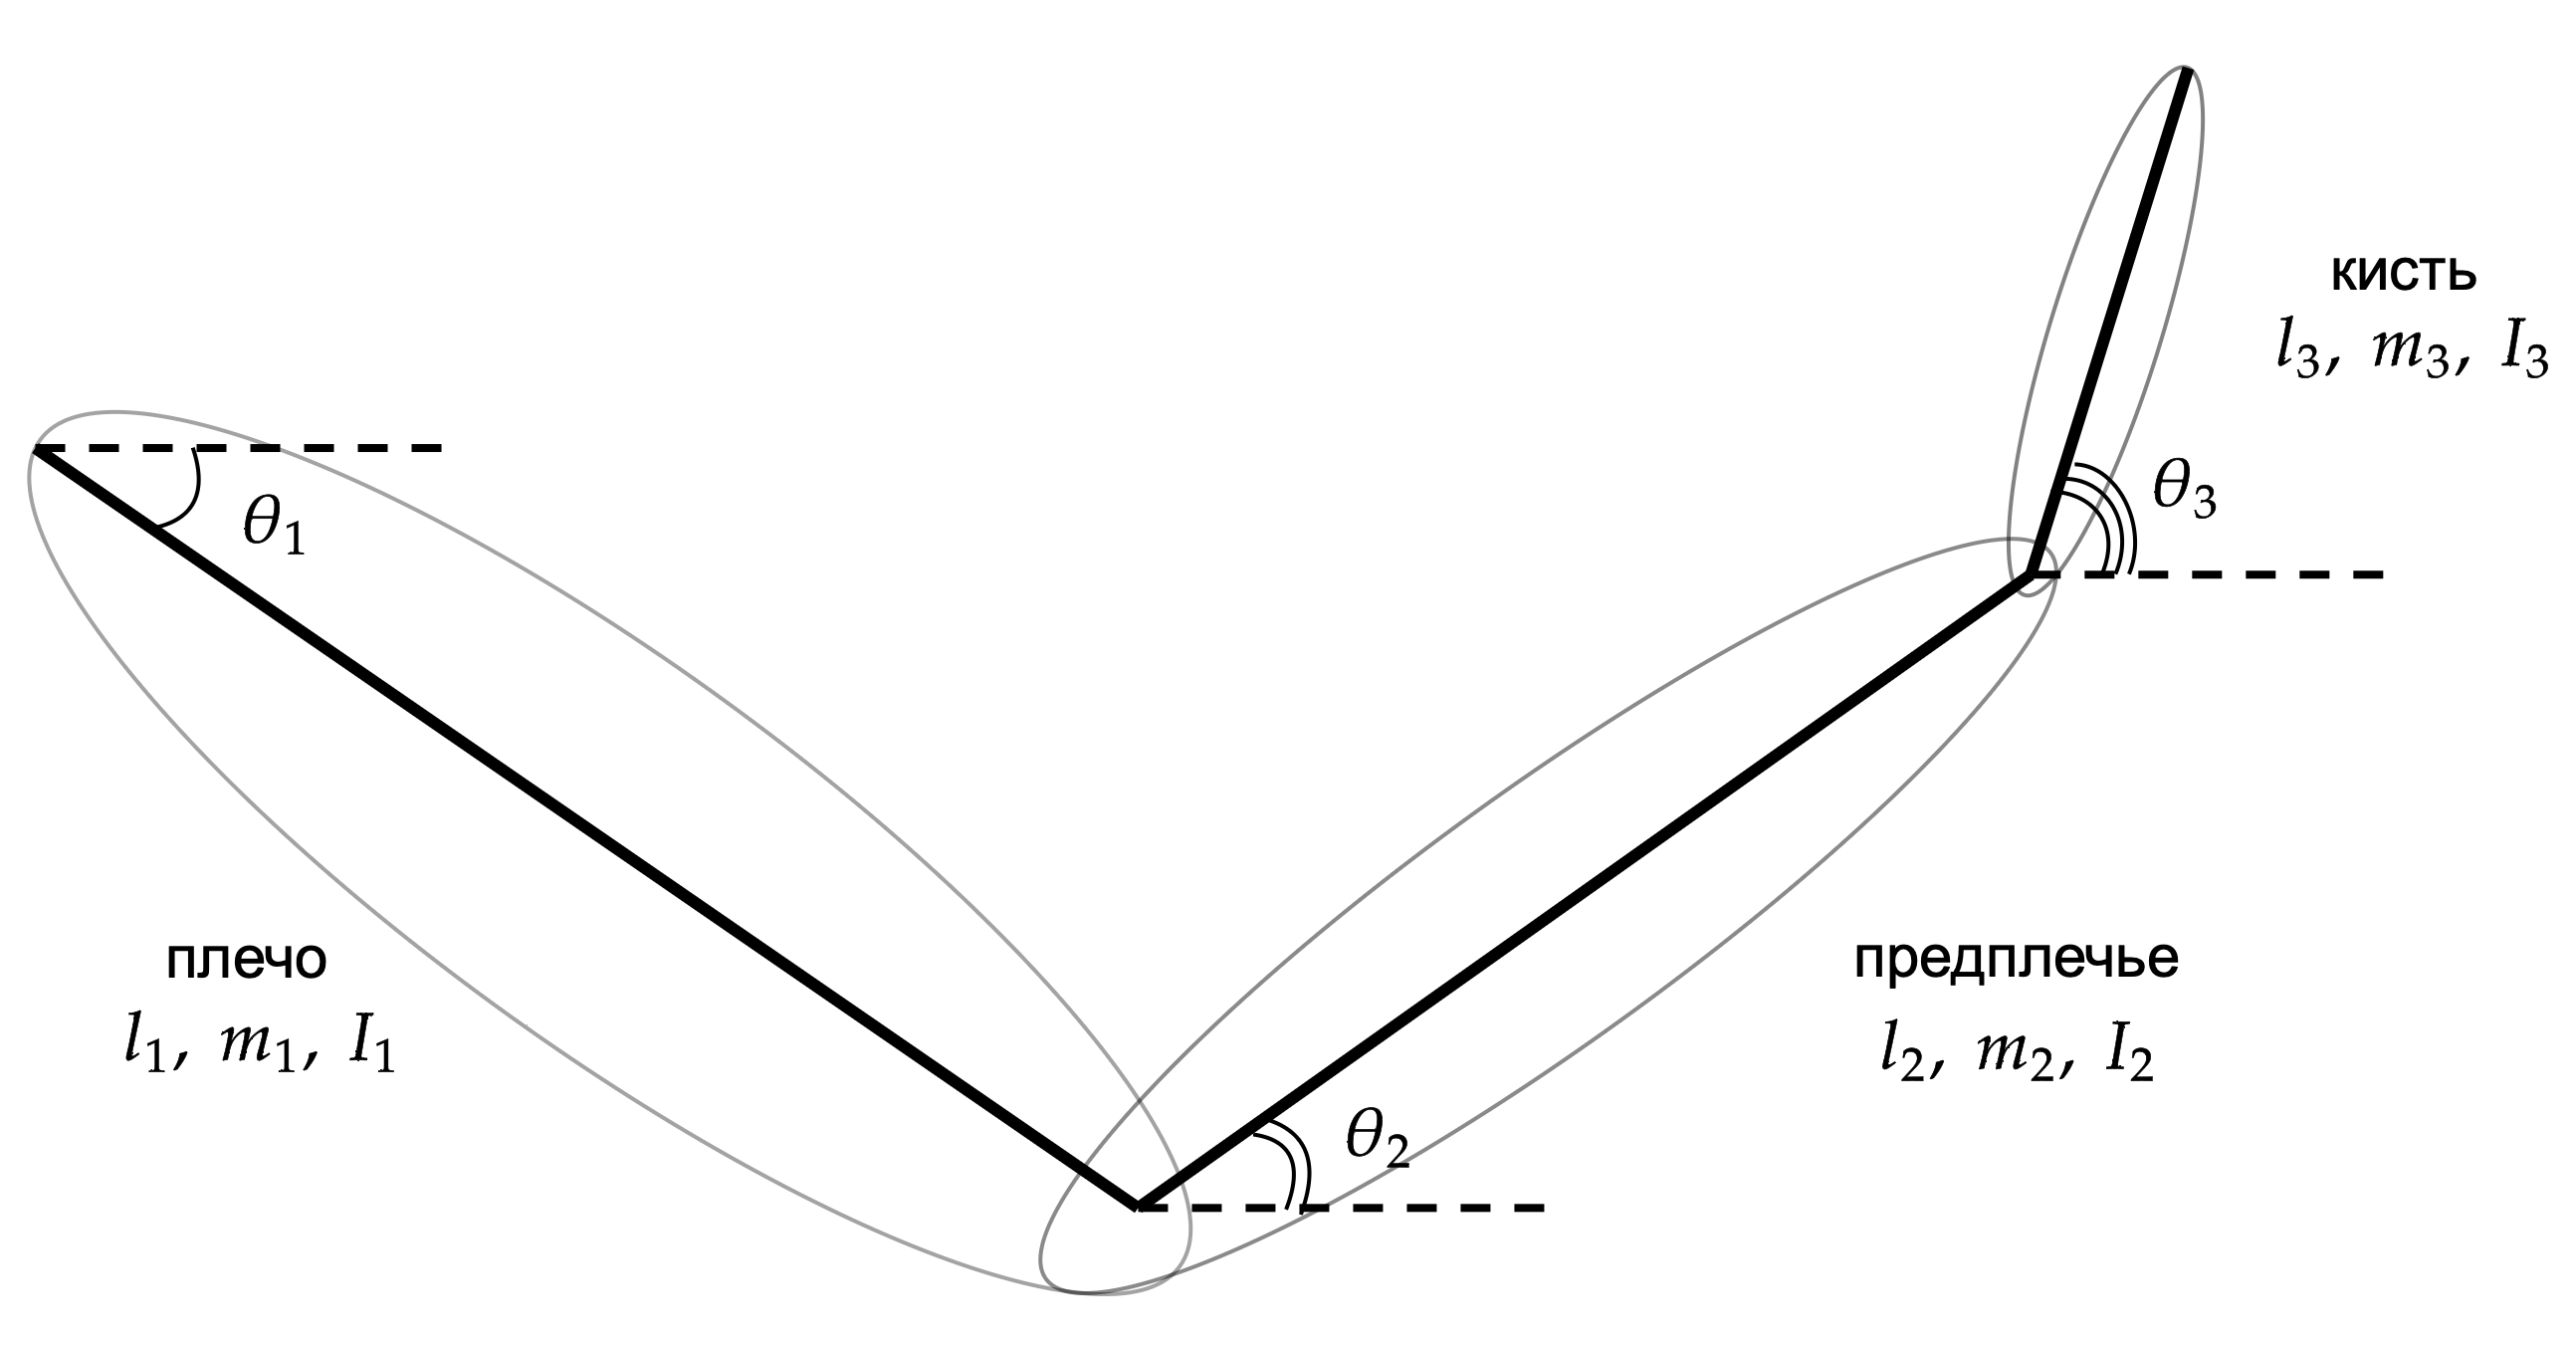
\includegraphics[width=0.8\textwidth]{img/arm.png}
        }
        \begin{block}{Начальные данные}
            \begin{itemize}
                \item Рука --- 3-х сочленённый математический маятник.
                \item Известны длины $\ell_i$, массы $m_i$ и моменты инерции $I_i$.
                \item Фазовые переменные --- углы поворота сочленения $\theta_i$ относительно оси $Ox$. 
            \end{itemize}
        \end{block}
    \end{frame}

    \begin{frame}{Математическое моделирование}
        Метод Эйлера--Лагранжа
        $$
            \mathcal{L} = \Pi - K
            \;\Longrightarrow\;
            \tau_i
            =
              \frac{d}{dt}\left(\frac{\partial \mathcal{L}}{\partial \dot \theta_i}\right)
            - \frac{\partial \mathcal{L}}{\partial \theta_i},
        $$
        где $K$ и $\Pi$ --- общие кинетическая и потенциальная энергии системы.
        \vfill
        \begin{block}{Уравнение динамики}
            $$
                \tau = M(\theta)\ddot\theta + L(\theta, \dot\theta)
            $$
            \begin{itemize}
                \item $\tau_i$~--- момент силы, действующей на $i$-е сочленение
                \item $M(\theta)=M^{\mathrm{T}}(\theta)>0$~--- матрица инерции
                \item $L(\theta, \dot\theta)$~--- вектор центростремительных и корелисовых сил
            \end{itemize}
        \end{block}
    \end{frame}

    \begin{frame}{Математическое моделирование}
        \begin{figure}
            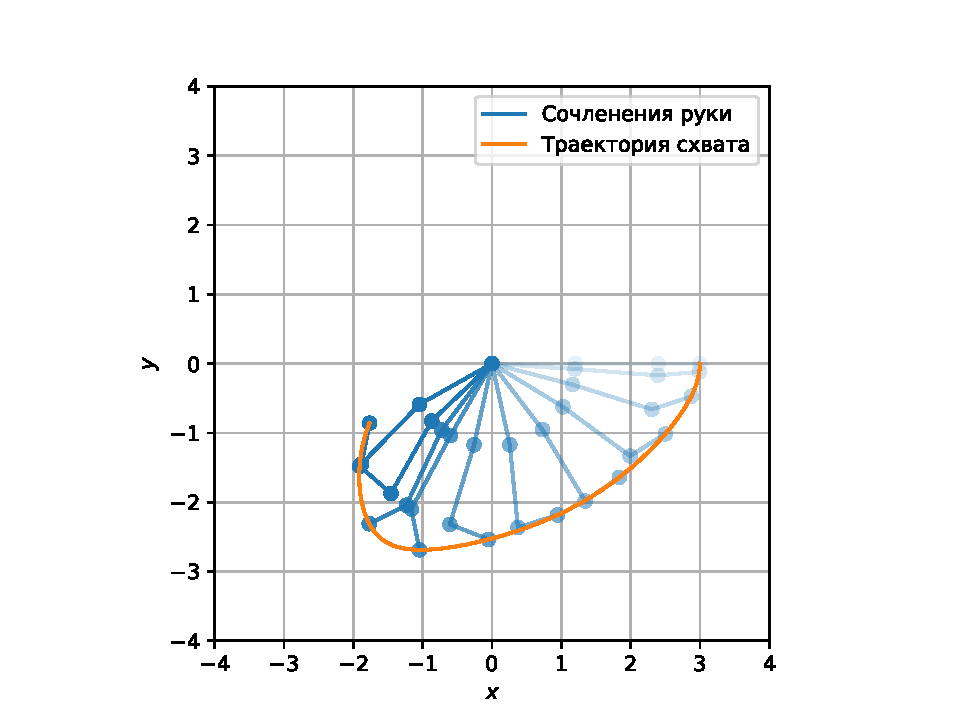
\includegraphics[width=0.8\textwidth]{img/discrete_pendulum.pdf}
            \caption{Траектория руки в свободном падении}
        \end{figure}
    \end{frame}

    \begin{frame}{Принцип оптимальности}
        \begin{itemize}
            \item Биологическое движение требует обработки большого количества информации
            \item Моторно-двигательная система как результат эволюции и обучения строит движение в соотвествии с принципом оптимальности
        \end{itemize}
        \vfill
        \begin{block}{Биологический принцип оптимальности}
            Выбираемые нервной системой схемы движения являются оптимальными для поставленной задачи.
        \end{block}
    \end{frame}

    \begin{frame}{Энергетические затраты}
        В работе [2] показано, что оптимизации проводится с целью уменьшения затрат энергии.
        \vfill
        \begin{block}{Формализация энергетических затрат [3]}
            $$
                \mbox{Затраты}\, = \int\limits_{t_{start}}^{t_{final}}\|\dot\tau\|^2\,dt
            $$
        \end{block}
    \end{frame}

    \begin{frame}{Задача достижения целевого положения}
        Введем $x = [\theta\;\dot\theta\;\tau]^{\mathrm{T}}$, тогда уравнение динамики примет вид
        $$
            \dot x = A(x) + Bu,\;
            \mbox{где}\,
            A(x) = \left[\begin{aligned}
                x_2 \\
                M^{-1}(x_1)(x_3 - L(x_1, x_2)) \\
                0
            \end{aligned}\right],
            B = \left[\begin{aligned}
                0 \\ 0 \\ 1
            \end{aligned}\right].
        $$
        Задано начальное положение:
        $$
            x(t_{start}) = x^{start}
        $$
        Задача минимизации функционала:
        $$
            J = w_1
            \underbrace{\langle x-x^{final}, x-x^{final} \rangle}_{Q^{final}(x)} + w_2 \int\limits_{t_{start}}^{t_{final}}\underbrace{\langle u, u\rangle}_{Q(x, u)}\,dt \longrightarrow \mathrm{min}
        $$
    \end{frame}

    \begin{frame}{Дискретизация задачи}
        Введем сетку по переменной $t = \{t_k\}_{k = 1}^{N+1}$ с шагом $\Delta t$ и дискретизируем задачу:
        $$
            \left\{
            \begin{aligned}
            &x^{k+1} = f(x^k, u^k) \\
            &x^0 = x^{start},
            \end{aligned}
            \right.
        $$
        где $f(x^k, u^k) = \Delta t [A(x^k) + Bu^k] + x^k$.
        $$
            J = Q^{N+1}(x^{N+1}) + \sum_{k=1}^{N} Q^{k}(x^k, u^k)\;\longrightarrow\;\mathrm{min},
        $$
        где $Q^{k}(x^k, u^k) = w_2 \Delta t Q(x^k, u^k)$, $Q^{N+1}(x^{N+1}) = w_1Q^{final}(x^{N+1})$.
    \end{frame}

    \begin{frame}{Дифференциальное динамическое программирование}
        \begin{block}{Идея метода}
            \begin{itemize}
                \item Берётся некоторое \textit{референсное} допустимое управление $u$ и соответствующая ей референсная траектория $x$
                \item Задача управления решается точно на каждой итерации алгоритма для коррекции референсного управления с целью снижения значения функции цены
                \item Используя информацию о градиенте гамильтониана $H$ на референсной траектории строится поправка вида
                $$
                    \Delta u = \eta \nabla_u H(u)
                $$
                \item Если решение не удовлетворяет заданной точности $\varepsilon$, получившееся управление берется в качестве референсного для следующей итерации алгоритма 
            \end{itemize}
        \end{block}
    \end{frame}

    \begin{frame}{Дифференциальное динамическое программирование}
        Пусть $(u, x)$~--- управление и соответствующая ему траектория на предыдущем шаге алгоритма. Рассмотрим Гамильтониан:
        $$
            H = Q_{N+1}(x^{N+1}) + \sum_{k=0}^N Q_k(x^k, u^k) + \sum_{k=0}^{N}\lambda_k^{\mathrm{T}}(x^{k+1} - f(x^k, u^k))
        $$
        \begin{block}{Необходимые условия оптимальности 1-ого порядка}
            \begin{align*}
                \frac{\partial H}{\partial \lambda_k} = x_{k+1} - f(x_k, u_k) &= 0 \\
                \frac{\partial H}{\partial x^k} = \frac{\partial Q_k}{\partial x}(x^k,u^k) - \frac{\partial f}{\partial x}^{\mathrm{T}}(x^k, u^k)\lambda_k + \lambda_{k-1} &= 0 \\
                \frac{\partial H}{\partial x^{N+1}} = \frac{\partial Q_{N+1}}{\partial x}(x^{N+1}) + \lambda_{N} &= 0 \\
                \frac{\partial H}{\partial u^k} = \frac{\partial Q_k}{\partial u}(x^k, u^k) - \frac{\partial f}{\partial u}^{\mathrm{T}}(x^k, u^k)\lambda_k &= 0
            \end{align*}
        \end{block}
    \end{frame}

    \begin{frame}{Дифференциальное динамическое программирование}
        \begin{enumerate}
            \item Рассчитать $\lambda_k$ для $k=N,\,N-1,\,\ldots,\,1$:
            
            $
                \begin{aligned}
                    &\lambda_N = - \frac{\partial Q_{N+1}}{\partial x}(x^{N+1})\\
                    &\lambda_{k-1} = \frac{\partial f}{\partial x^k}^{\mathrm{T}}(x^k, u^k)\lambda_k - \frac{\partial Q_k}{\partial x}(x^k, u^k)
                \end{aligned}
            $
            
            \item Рассчитать $\frac{\partial H}{\partial u_k}$ для $k=N,\,N-1,\,\ldots,\,1$:
            
            $
                \frac{\partial H}{\partial u_k} = \frac{\partial Q_k}{\partial u}(x^k, u^k) - \frac{\partial f}{\partial u}^{\mathrm{T}}(x^k, u^k)\lambda_k
            $

            \item Сделать поправку на исходную траекторию $u_k$, прибавив к ней поправку $\Delta u_k = -\eta\frac{\partial H}{\partial u_k}$,
            где коэффициент $\eta$ выбирается таким образом, чтобы получившееся управление было допустимым, то есть $u_k + \Delta u_k \in \mathcal{U}$.
            \item Остановить алгоритм в случае, если $\sum_{k=0}^n \left\| \frac{\partial H}{\partial u_k} \right\|^2 < \varepsilon$.
        \end{enumerate}
    \end{frame}

    \begin{frame}{Дифференциальное динамическое программирование}
        \begin{figure}
            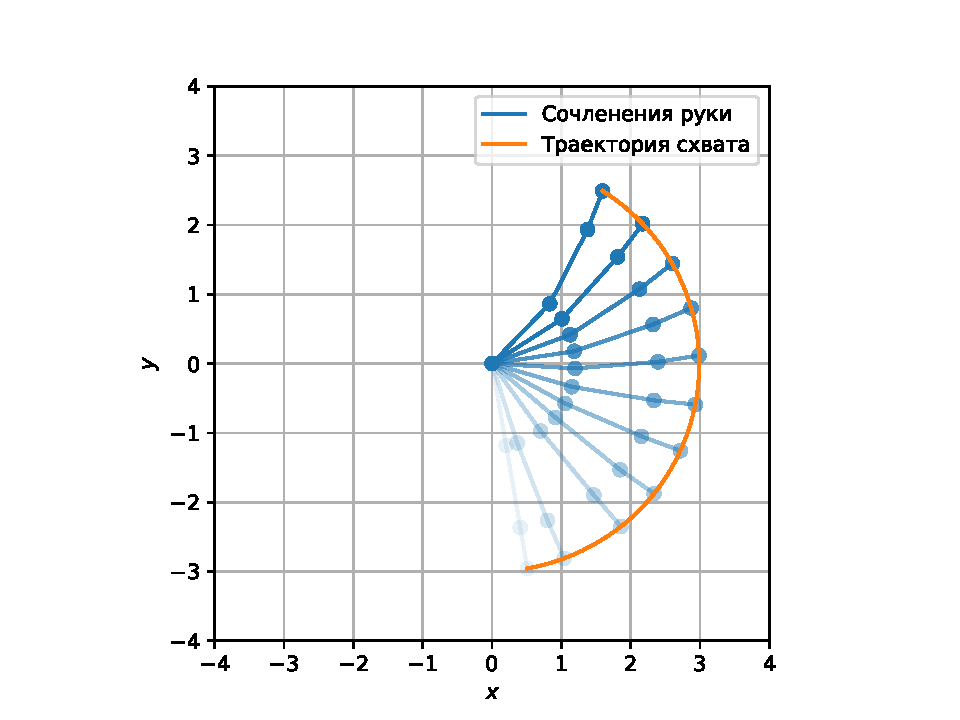
\includegraphics[width=0.8\textwidth]{img/ddp_pendulum.pdf}
            \caption{Траектория руки, построенная методом ДДП.}
        \end{figure}
    \end{frame}

    \begin{frame}{Дифференциальное динамическое программирование}
        \begin{figure}
            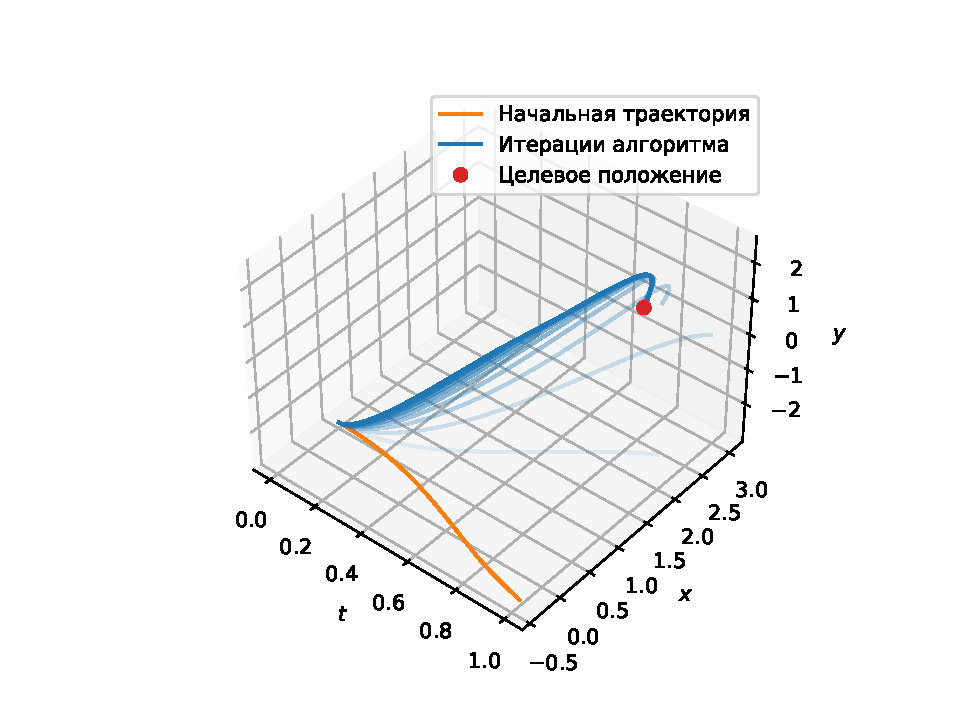
\includegraphics[width=0.8\textwidth]{img/ddp_empty.pdf}
            \caption{Траектории схвата для итеративного алгоритма при нулевом начальном управлении $u^{ref}\equiv 0$. Показана каждая 3-я итерация.}
        \end{figure}
    \end{frame}
    
    \begin{frame}{Референсная траектория}
        \begin{block}{Мотивация}
            \begin{itemize}
                \item Градиентный метод сходится довольно долго
                \item Мы хотим выбрать начальное референсное управление таким образом, чтобы оно частично удовлетворяло условию задачи, с целью сократить число итераций алоритма
                \item Это управление должно \textit{быстро} строиться
                \item Оно должно быть допустимым для рассматриваемой задачи
            \end{itemize}
        \end{block}
    \end{frame}

    \begin{frame}{Референсная траектория}
        Приведем систему к линейной, заменой управления
        $$
            v = M^{-1}(x_1)(\tau - L(x_1, x_2))
        $$
        Тогда система примет вид:
        \begin{equation}\label{eq:linear}
            x^{k+1} =  \underbrace{\mathrm{diag}\{I,O\}}_{A_{ref}} x^{k} + \underbrace{\mathrm{diag}\{O, I\}}_{B_{ref}} v^{k}
        \end{equation}

        Решим для системы \eqref{eq:linear} задачу минимизации интегрально-квадратичного функционала:
        $$
            J^{ref} = \langle (x-x^{final}), T^{final}(x-x^{final}) \rangle + \sum_{k=1}^{N} \langle v^k, Tv^k \rangle \longrightarrow \mathrm{min}
        $$

        Получим референсное управление $u$ из соотношения
        $$
            \tau^k = M(x_1^k)v^k + L(x_1^k,x_2^k) \;\Longrightarrow\; u^{k} = \frac{\tau^{k+1} - \tau^{k}}{\Delta t}
        $$
    \end{frame}

    \begin{frame}{Референсная траектория}
        Метод динамического программирования даёт решение данной задачи:
        $$
            v^k_* = -[T + B_{ref}^{\mathrm{T}}P^kB_{ref}]^{-1}P^kB_{ref}A_{ref} x,
        $$
        где матрица $P^k$ может быть посчитана в обратном времени как решение уравнения Риккати:
        $$
            \begin{aligned}
                &P^{k-1} = A_{ref}^{\mathrm{T}} P^{k} A_{ref} - A_{ref}^{\mathrm{T}}P^kB_{ref}[T + B_{ref}^\mathrm{T}P^kB_{ref}]^{-1}B_{ref}^{\mathrm{T}}P^{k}A_{ref}
                \\
                &P^{N+1} = T^{final}
            \end{aligned}
        $$
        \begin{block}{Полученное управление}
            \begin{itemize}
                \item Считается за одну итерацию
                \item Минимизирует изменение углового ускорения, значит, допустимо
                \item Приводит нас к целевому положению, но ничего не говорит об энергии
            \end{itemize}
        \end{block}
    \end{frame}

    \begin{frame}{Референсная траектория}
        \begin{figure}
            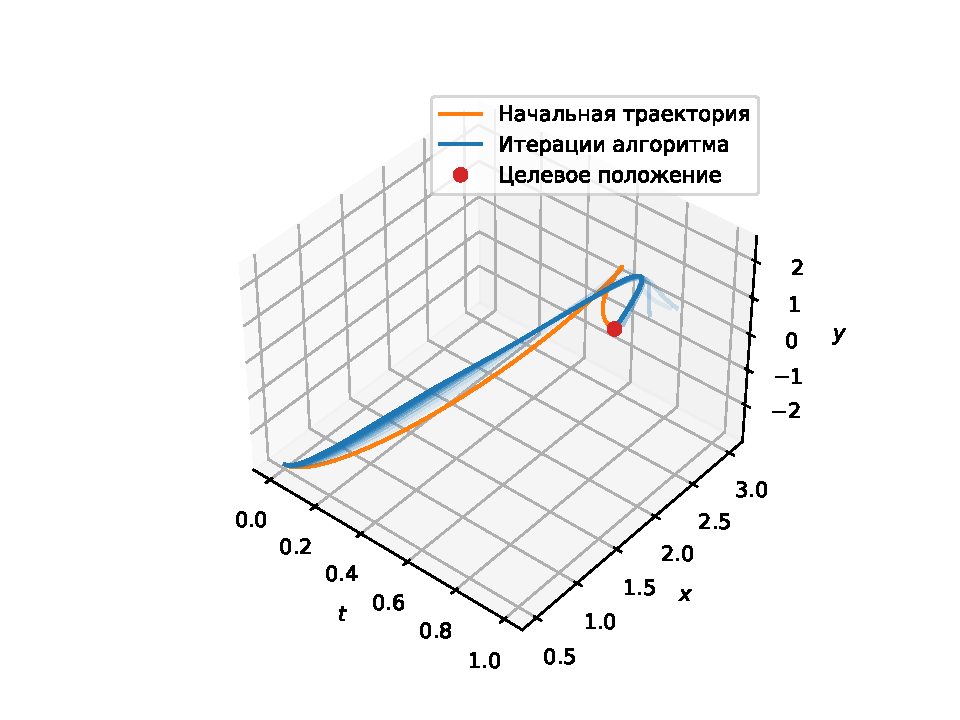
\includegraphics[width=0.8\textwidth]{img/ddp_dummy.pdf}
            \caption{Траектории схвата для итеративного алгоритма при новом начальном управлении. Показана \textit{КАЖДАЯ} итерация.}
        \end{figure}
    \end{frame}

    \begin{frame}{Пример [Обход препятствий]}
        Добавим компонент в функцию цены:
        $$
            J_{\,\mbox{\small{преп}}} = w_3 \int_{t_{start}}^{t_{final}} \left(\| e_{\,\mbox{\small{схв}}} - e_{\,\mbox{\small{преп}}} \|^2 - r_{\,\mbox{\small{преп}}}\right)^{-2}\,dt,
        $$
        где
        \begin{itemize}
            \item $e_{\,\mbox{\small{схв}}}$ --- положение схвата
            \item $e_{\,\mbox{\small{преп}}}$ --- центр препятствия
            \item $r_{\,\mbox{\small{преп}}}$ --- радиус препятствия
        \end{itemize}
        \vfill
        Далее будем пользоваться алгоритмом.
    \end{frame}

    \begin{frame}{Пример [Обход препятствий]}
        \begin{figure}
            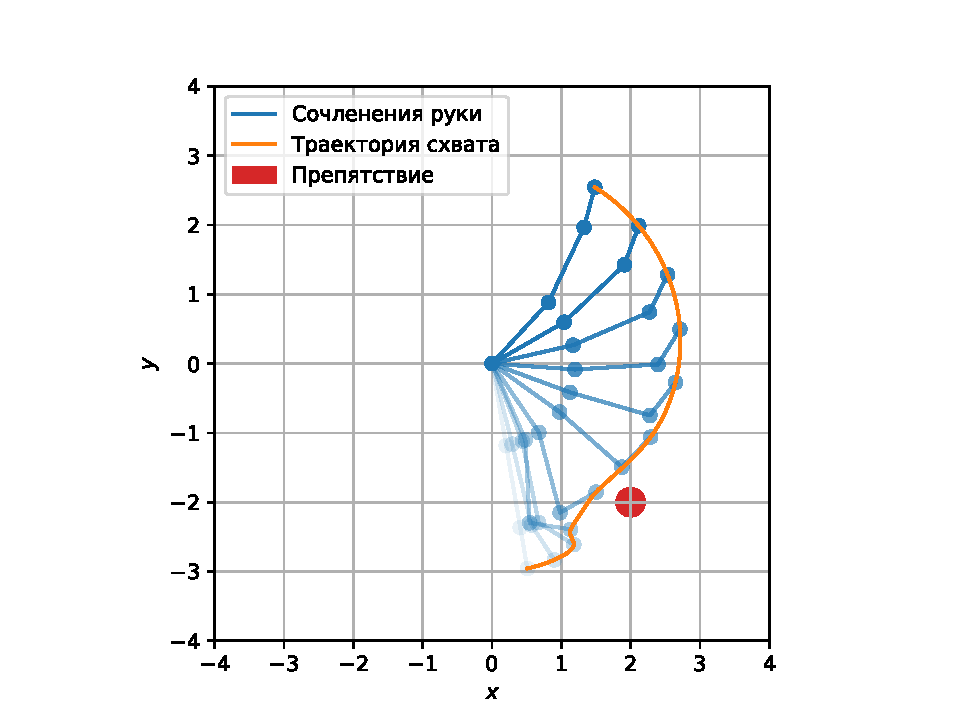
\includegraphics[width=0.49\textwidth]{img/obstacle_pendulum.pdf}
            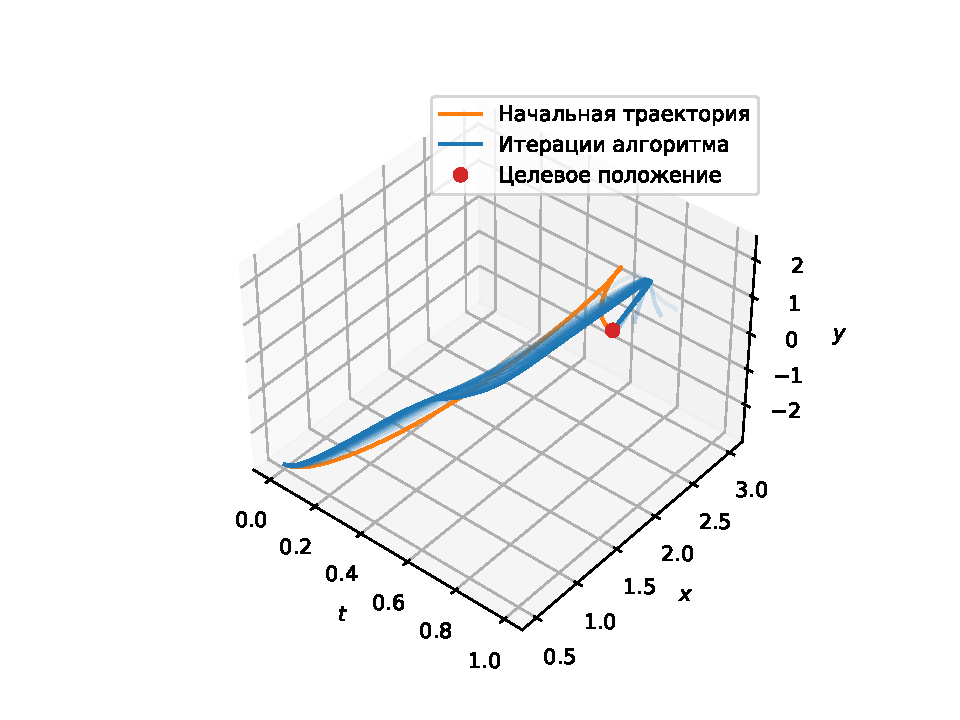
\includegraphics[width=0.49\textwidth]{img/ddp_obstacle.pdf}
            \caption{Траектории руки и схвата для задачи обхода препятствия}
        \end{figure}
    \end{frame}

    \begin{frame}{Список литературы}
        \begin{enumerate}
            \item[1] Колюбин~С.\,А. Динамика робототехнических систем~// Учебное пособие. --- СПб.: Университет ИТМО, 2017.~--- 117 с.
            \item[2] E. Todorov, M. Jordan. Optimal feedback control as a theory of motor coordination~// Nature Neuroscience, Vol.5, No.11, 1226-1235, 2002.
            \item[3] Y. Uno, M. Kawato, R. Suzuki. Formation and control of optimal trajectory in human multijoint arm movement~--- minimum torque-change model~// Biological Cybernetics 61, 89-101, 1989.
            \item[4] B.D.O. Anderson, J.B. Moore. Optimal Control: Linear Quadratic Methods~// Prentice Hall, Upper Saddle River, 1990.
            \item[5] D. H. Jacobson. Differential dynamic programming methods for determining optimal control of non-linear systems~// University of London, 1967.
        \end{enumerate}
    \end{frame}

    \begin{frame}{Список литературы}
        \begin{enumerate}
            \item[6] E. Guechi, S. Bouzoualegh, Y. Zennir, S. Blažič. MPC Control and LQ Optimal Control of A Two-Link Robot Arm: A Comparative Study~// Machines 6, no. 3: 37, 2018.
            \item[7] A. Babazadeh, N. Sadati. Optimal control of multiple-arm robotic systems using gradient method~// IEEE Conference on Robotics, Automation and Mechatronics, Singapore, pp. 312-317 vol.1, 2004.
        \end{enumerate}
    \end{frame}
\end{document}